\chapter{Background}
\label{sec:background}

\vspace{1cm} % Optional: Adjust this to add more space below the chapter title if needed
\begin{center}
\centering
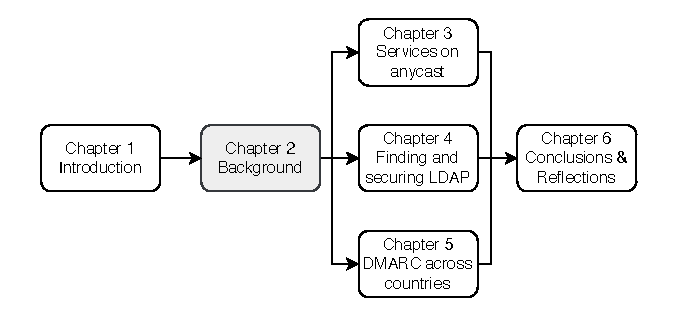
\includegraphics[width=\textwidth]{figures/thesis-schematic-background.pdf}
\end{center}

\emph{This chapter provides background information on Anycast, \gls{tls}, \gls{ldap}, and email security protocols such as \gls{spf}, \gls{dkim}, and \gls{dmarc}.
This information is necessary to to understand the subsequent chapters.
Our goal is not to provide an exhaustive description of the aforemetioned topics, but rather offer sufficient details relevant to this thesis.}

\newpage

\section{Anycast}
\label{sec:background-anycast}
When a user connects to an anycast address, \gls{bgp} directs the request to a single \gls{pop},
typically one that is topologically close to the user~\cite{rfc4786}, from which the service replies.
%
A common misconception is that announcing an address at multiple locations, in itself, is classified as anycast.
Many \glspl{cdn} announce their prefixes at multiple network edges (in different geographic regions),
where they route traffic internally to a single \gls{pop} hosting the service.
Critically, as defined in RFC~4786~\cite{rfc4786},
anycast is the replication of a service address where several \glspl{pop} make the service available.

\section{TLS}

\section{LDAP}

\section{Email Security Protocols}

\subsection{DKIM}
\subsection{SPF}
\subsection{DMARC}
